\documentclass{article}
	\usepackage[utf8]{inputenc}
	\usepackage{float}
	\usepackage{pdfpages}
	\usepackage[T1]{fontenc}
	\usepackage{float}
	\usepackage{booktabs}
	\usepackage{multirow}
	\usepackage{ragged2e}
	\usepackage{makecell}
	\renewcommand{\theadfont}{\small\bfseries}
	\usepackage{tabularx}
	\usepackage[autolanguage, np]{numprint}
	\newcolumntype{Z}{ >{\centering\arraybackslash}X }
	\usepackage{makecell}
	\usepackage{url}
	\usepackage{siunitx}
	\usepackage{caption}
	\usepackage[framemethod=TikZ]{mdframed}
	\usepackage{tikz, tabularx}
	\usepackage[T1]{fontenc}
	\usepackage{charter}

%%% Document Properties and Packages used 9/20
\usepackage{amsmath}        % math formulas
\usepackage{bm}             % bold math symbols
\usepackage{multicol}       % multiple columns
\usepackage[super]{nth}     % 1st, 2nd, 3rd, 4th
\usepackage{enumitem}       % ordered list (a), (b), (c)
\usepackage{graphicx}		% insert images
\graphicspath{ {./images/} }
\usepackage{geometry}
\geometry{letterpaper, margin=1in, top=0.5in} % small margins
\usepackage{biblatex}		% bibliography
\addbibresource{HW1N1.bib}
%%%%%%%%%%%%%%%%%%%%%%%%%%%%%%%%%%%%%%%%%%%%%%%%%%%%%%%%%%%%%%%%%%%%%%%%%%%%%%%
%%% Code Listing 
\usepackage{listings}
\usepackage{xcolor}

\definecolor{codegreen}{rgb}{0,0.6,0}
\definecolor{codegray}{rgb}{0.5,0.5,0.5}
\definecolor{codepurple}{rgb}{0.58,0,0.82}
\definecolor{backcolour}{rgb}{0.95,0.95,0.92}

\lstdefinestyle{mystyle}{
	backgroundcolor=\color{backcolour},   
	commentstyle=\color{codegreen},
	keywordstyle=\color{magenta},
	numberstyle=\tiny\color{codegray},
	stringstyle=\color{codepurple},
	basicstyle=\ttfamily\footnotesize,
	breakatwhitespace=false,         
	breaklines=true,                 
	captionpos=b,                    
	keepspaces=true,                 
	numbers=left,                    
	numbersep=5pt,                  
	showspaces=false,                
	showstringspaces=false,
	showtabs=false,                  
	tabsize=2
}
\lstset{style=mystyle}
%%%%%%%%%%%%%%%%%%%%%%%%%%%%%%%%%%%%%%%%%%%%%%%%%%%%%%%%%%%%%%%%%%%%%%%%%%%%%%%
\begin{document}
	
	\noindent\textbf{Justine John "JJ" A. Serdoncillo}
	\hfill \textbf{AEM 5253: Computational Fluid Dynamics} \\ \hfill \textbf{November 1, 2022}
	
	\begin{center}
		\Large{\textbf{Homework 2}}    
	\end{center}
	
	\section*{Number 1 b)}
	The figures below are the plots of the real and imaginary parts of the modified wave number.
	
	\begin{figure}[H]
		\centering
		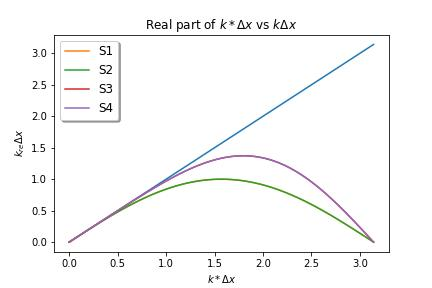
\includegraphics[width=0.6\textwidth]{real.jpg}
		\caption{\label{} Real part of the modified wave number }
	\end{figure}

	\begin{figure}[H]
		\centering
		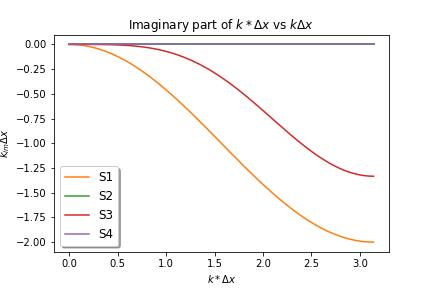
\includegraphics[width=0.6\textwidth]{imag.jpg}
		\caption{\label{} Imaginary part of the modified wave number }
	\end{figure}

	\section*{Number 1 c)}
	The figure below plots the percent error as the wave number is changed. It can be seen that the intersection values correspond to the limit wave number to get the desired accuracy. These numbers correspond to around 0.787 and 1.395 for the S2 and S4 schemes respectively.

	\begin{figure}[H]
		\centering
		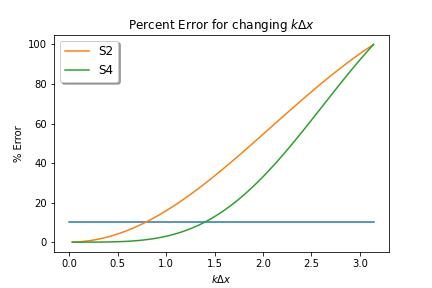
\includegraphics[width=0.6\textwidth]{error.jpg}
		\caption{\label{} Percent Error of the modified wave number }
	\end{figure}

	\section*{Number 3 a)}
	The figures below are the plots of the advection equation with the Gaussian function and square pulse equation as the two different initial conditions. The spatial schemes used were the ones in number 1 while the time stepping scheme used is Runge-Kutta 3rd order. 
	
	\begin{figure}[H]
		\centering
		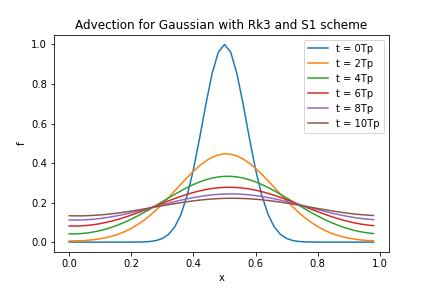
\includegraphics[width=0.6\textwidth]{ad1.jpg}
		\caption{\label{} Gaussian advection using Rk3 and S1}
	\end{figure}
	\begin{figure}[H]
		\centering
		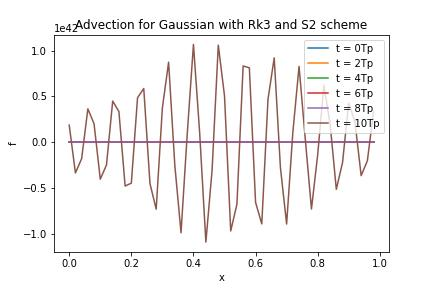
\includegraphics[width=0.6\textwidth]{ad2.jpg}
		\caption{\label{} Gaussian advection using Rk3 and S2}
	\end{figure}
	\begin{figure}[H]
		\centering
		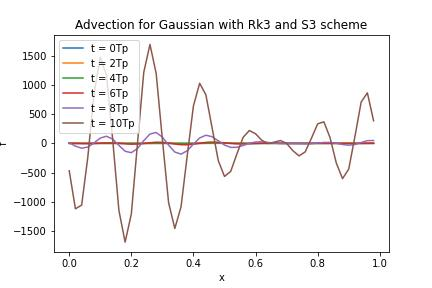
\includegraphics[width=0.6\textwidth]{ad3.jpg}
		\caption{\label{} Gaussian advection using Rk3 and S3}
	\end{figure}
	\begin{figure}[H]
		\centering
		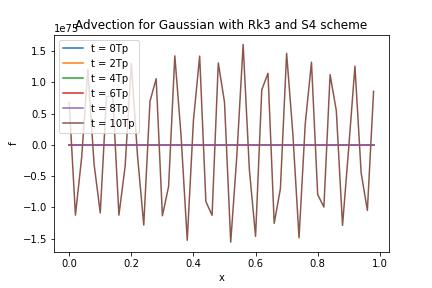
\includegraphics[width=0.6\textwidth]{ad4.jpg}
		\caption{\label{} Gaussian advection using Rk3 and S4}
	\end{figure}

	\begin{figure}[H]
		\centering
		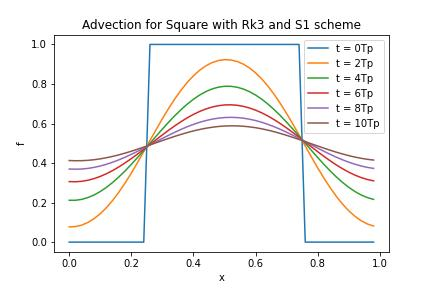
\includegraphics[width=0.6\textwidth]{ad5.jpg}
		\caption{\label{} Square Pulse advection using Rk3 and S1}
	\end{figure}
	\begin{figure}[H]
		\centering
		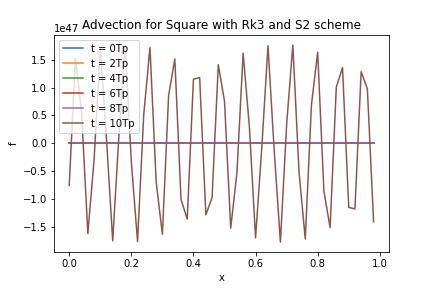
\includegraphics[width=0.6\textwidth]{ad6.jpg}
		\caption{\label{} Square Pulse advection using Rk3 and S2}
	\end{figure}
	\begin{figure}[H]
		\centering
		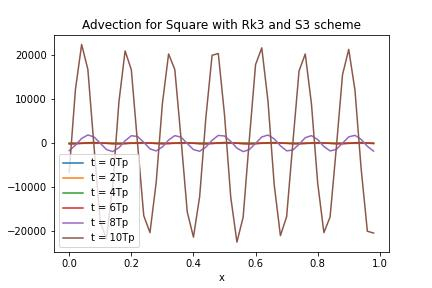
\includegraphics[width=0.6\textwidth]{ad7.jpg}
		\caption{\label{} Square Pulse advection using Rk3 and S3}
	\end{figure}
	\begin{figure}[H]
		\centering
		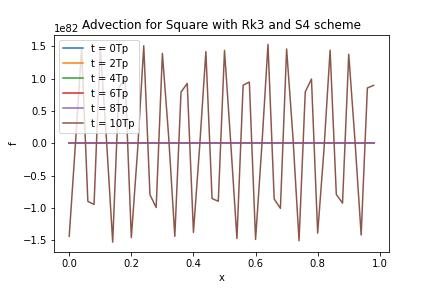
\includegraphics[width=0.6\textwidth]{ad8.jpg}
		\caption{\label{} Square Pulse advection using Rk3 and S4}
	\end{figure}
	
	\section*{Number 3 b)}
		From the figures above, it can be seen that most of the plots have a pretty random oscillating solution at the higher time steps. However, the S1 schemes produced clear plots but the amplitude decreases as time increases. This is as shown in class as dissipation in the S1 schemes.
		\\
		Another notable thing can be seen is through the S3 scheme because the oscillation is non-uniform and there is a change in size of the amplitude as well. By only plotting the first few Tp, we find the figure below. It can be seen that there are now waves beside the main wave. This is explained in class as dispersion and the increase in amplitude can be attributed to diffusion. The stencil is biased towards the left which explains why the dispersion is asymmetric. 
		
		\begin{figure}[H]
			\centering
			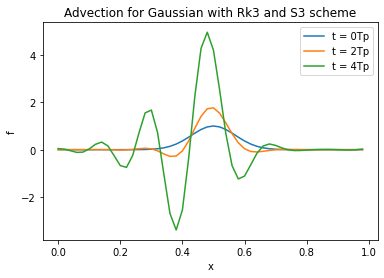
\includegraphics[width=0.6\textwidth]{ad3extra.png}
			\caption{\label{} Gaussian showing clear Dispersion}
		\end{figure}
	
		Lastly, S2 and S4 are both central order schemes which in class discussion is not ideal because the eigenvalues are all imaginary and adds some positive diffusion. This is clearly shown as the plots look pretty random with the large oscillations. 
	
\end{document}
